\documentclass[a4paper, 12pt]{article}

\title{Battleships}
\author{Carl Sandrock}

\usepackage{graphicx}
\usepackage{booktabs}
\usepackage[hang, small, bf]{caption}
\usepackage[margin=1.1in]{geometry}

\newcommand\matlab{{\scshape Matlab}}

\begin{document}
%\maketitle
\begin{centering}
\Huge Battleships \\
\end{centering}

\section{The game}
You will be writing a program that will play one half of a game of
battleships.  You only have to guess the positions of a hidden fleet
of ships, but will not place any ships of your own.

In our version of battleships the game starts with the computer
secretly placing a fleet of 5 ships on a 10$\times$10 grid as shown
below.  The positions of the ships are fixed, but unknown to you.

\begin{figure}[htbp]
  \setlength{\unitlength}{0.75cm}
  \centering
  \begin{picture}(11, 11)
    % Grid lines
    \multiput(0, 0)(1, 0){11}{\line(0, 1){10}}
    \multiput(0, 0)(0, 1){11}{\line(1, 0){10}}
    % Left numbers
    \put(-1,9.3){1}
    \put(-1,8.3){2}
    \put(-1,7.3){3}
    \put(-1,6.3){4}
    \put(-1,5.3){5}
    \put(-1,4.3){6}
    \put(-1,3.3){7}
    \put(-1,2.3){8}
    \put(-1,1.3){9}
    \put(-1,0.3){10}
    % Top numbers
    \put(0.3,10.3){1}
    \put(1.3,10.3){2}
    \put(2.3,10.3){3}
    \put(3.3,10.3){4}
    \put(4.3,10.3){5}
    \put(5.3,10.3){6}
    \put(6.3,10.3){7}
    \put(7.3,10.3){8}
    \put(8.3,10.3){9}
    \put(9.3,10.3){10}
    % Ships 2 3 3 4 5
    \linethickness{0.5\unitlength}
    \put(2.5, 8){\line(0, 1){2}}
    \put(3, 5.5){\line(1, 0){3}}
    \put(3.5, 6){\line(0, 1){3}}
    \put(2, 3.5){\line(1, 0){4}}
    \put(8.5, 2){\line(0, 1){5}}
  \end{picture}
  \caption{A valid starting grid in a game of battleships}
  \label{fig:startinggrid}
\end{figure}

The fleet is made up of
\begin{itemize}
\item \rule{2em}{0.5em} one 2 block ship 
\item \rule{3em}{0.5em}, \rule{3em}{0.5em} two 3 block ships, 
\item \rule{4em}{0.5em}, one 4 block ship
\item \rule{5em}{0.5em}, one 5 block ship 
\end{itemize}

The ships are placed as follows:
\begin{itemize}
\item Ships can only lie \emph{horizontally or vertically}, but not diagonally.
\item Ships must lie \emph{entirely within the grid}.
\item Ships \emph{cannot cross one another} (no two ships can occupy the same
  block)
\item Different ships \emph{may occupy adjacent blocks}.
\item Ships are \emph{placed randomly}.
\end{itemize}

As the game progresses you try to sink all of the computer's ships by
guessing where they are.  Each guess is called a ``shot'' and is aimed
at a (row, column) coordinate.  The computer will respond by
indicating whether the shot was a hit or a miss.  For example, a shot
at position (7,~3) would register a hit on our example grid in
figure~\ref{fig:startinggrid}, while a shot at position (9,~6) would
register a miss.  

If all the blocks that a ship occupies have been shot, the ship is
sunk and the computer will indicate this in addition to the normal
indication of a hit.  Thus, if positions (1,~3) and (2,~3) were both
shot, the computer would respond after the second shot by indicating
that a ship of length 2 has been sunk and which blocks it occupied.
As soon as the final ship is sunk, the game ends.  The object of a
game is to use as few guesses as possible.

\section{Computer implementation}
You will be supplied with a file called \verb|battle.m|.  This
\matlab\ function handles the placement of a fleet of ships responds
to shots as described above.  To start a game, run
\verb|battle('init')|.  You may now start to shoot at coordinates by
calling \verb|battle(r, c)| where \verb|r| and \verb|c| are a row and
column coordinate to shoot at.  The function will return two values
(\verb|result| and \verb|value|), the meaning of which are described
in table~\ref{tab:outputvars}:
\begin{table}[htbp]
  \centering
  \caption{Meaning of output variables of the battle function}
  \label{tab:outputvars}
  \begin{tabular}{ccl}
    \toprule
    \verb|result| & \verb|value| & Meaning \\
    \midrule
    -1 & \verb|[]| & Duplicate shot \\
    0 & \verb|[]| & Miss \\
    1 & \verb|[]| & Hit, no ship sunk \\
    1 & N$\times$2 matrix & Ship of length N sunk \\
    2 & scalar & All ships sunk.  \verb|value| contains number of
    shots. \\
    \bottomrule
  \end{tabular}
\end{table}

Calling \verb|battle('finish')| causes the function to return two
outputs -- \verb|finished|, which is zero if all the ships have not
been sunk, and \verb|shots|, which is the number of shots fired during
this game.

If \verb|battle('init', 1)| is used, a graphical representation of the
state of the game as it progresses will be generated.  Note that a
small delay is added if the graphics are enabled.  This causes an
animation effect.  The graphical representation uses a white dot to
indicate a missed shot and a red dot to indicate a hit.  When a ship
is sunk, a line is drawn through all the points where that ship was.

\section{Program requirements}
You must write a function called \verb|findships| that will be called
without arguments \emph{after} the game has been initialised and will
play the game of battleships.  An example session may look like this
(the graphical output generated by this run is shown in
figure~\ref{fig:sampleoutput}):

\begin{verbatim}
>> battle('init', 1);
>> findships
>> [finished, shots] = battle('finish')
finished =
     1
shots =
     50
\end{verbatim}

\begin{figure}[htbp]
  \centering
  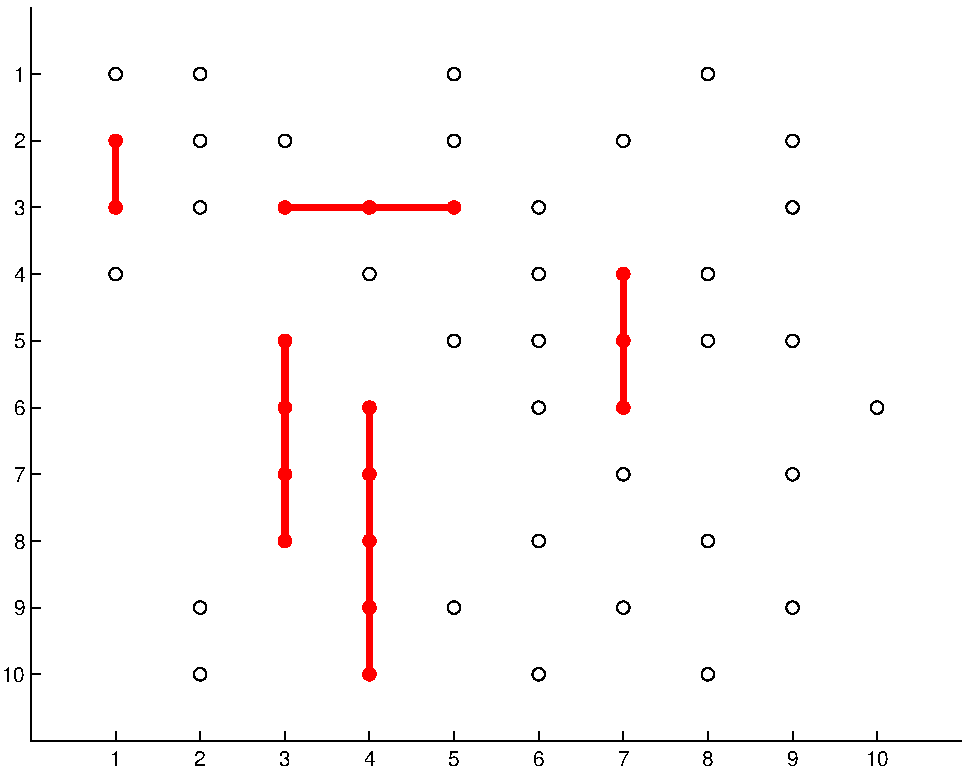
\includegraphics[width=0.8\textwidth]{sample}
  \caption{Sample graphics after a complete game}
  \label{fig:sampleoutput}
\end{figure}

Note that the default behaviour of your program should be to generate
\emph{no output} to the screen.  Any debugging messages should be
disabled before handing the program in.  Your program must terminate
when it has sunk all the ships (when \verb|battle| returns 2).

\section{Testing your program}
To help you determine the efficacy of your program, you will be
supplied with a function called \verb|testfindships|, which will run
\verb|findships| a certain number of times and display statistics
about the runs.  A sample run is shown below:

\begin{verbatim}
>> testfindships(500);
  run   min     avg   max   avg time (miliseconds)
  100    36    56.0    96       88
  200    36    55.0    96       86
  300    31    54.1    96       84
  400    31    54.9    99       86
  500    31    55.2    99       87
\end{verbatim}

The function shows the number of runs completed, the minimum, the
average and the maximum guesses required to find the ship, and the
average time per run that the \verb|findships| function required.
Note that \verb|testfindships| will output a vector containing the
exact results for each game for further analysis.

For instance, you could use the output of \verb|testfindships| to draw
a histogram showing the distribution of your results:

\begin{verbatim}
>> t = testfindships(1000);
>> hist(t)
\end{verbatim}
Output is shown in figure~\ref{fig:histogram}

\begin{figure}[htbp]
  \centering
  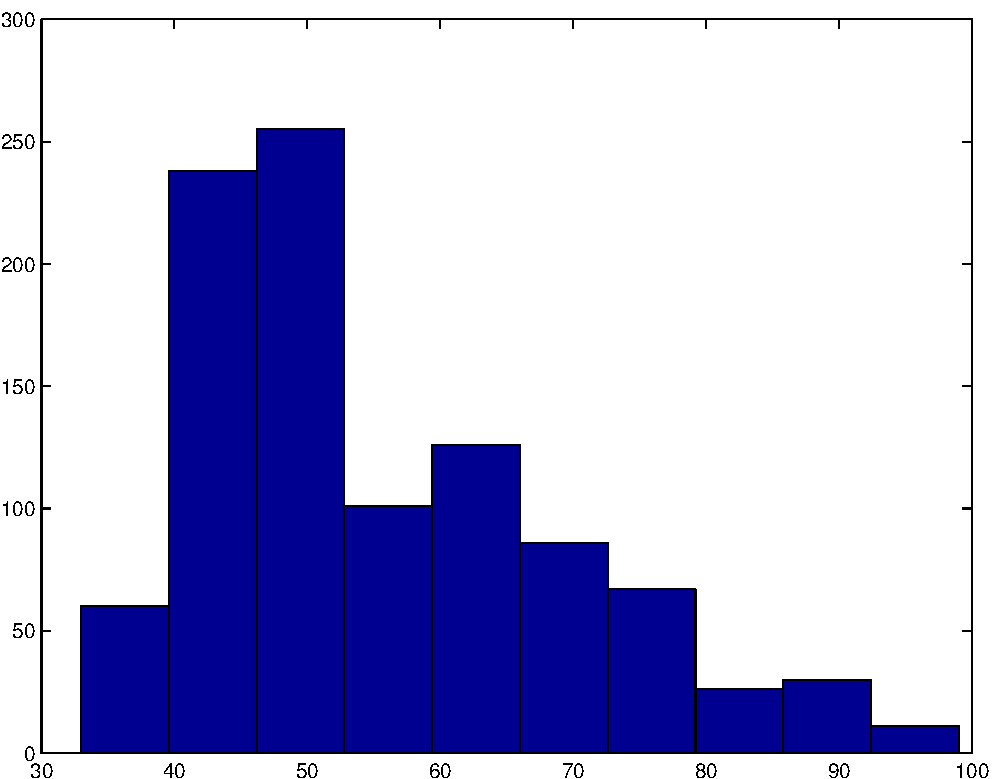
\includegraphics[width=0.7\textwidth]{battlehist}\\
  \caption{Histogram of guesses taken over 500 games}
  \label{fig:histogram}
\end{figure}

\section{Summary}
You will be supplied with the following files:\bigskip

\begin{tabular}{lll}
\toprule
Filename & Call  & Purpose \\
\midrule
\verb|battle.m| & \verb|battle('init')| & set up board without
graphics \\
& \verb|battle('init', 1)| & set up board with graphics \\
& \verb|battle(r, c)| & fire a shot at row \verb|r|, column \verb|c| \\
& \verb|battle('finish')| & determine status of game \\ 
\verb|testfindships.m| & \verb|testfindships(N)| & simulate \verb|N| games of
battleships \\
\bottomrule
\end{tabular}\bigskip

You must submit a file called \verb|findships.m|, which will be called
without arguments and call \verb|battle| to fire shots.

\end{document}
